% Options for packages loaded elsewhere
\PassOptionsToPackage{unicode}{hyperref}
\PassOptionsToPackage{hyphens}{url}
%
\documentclass[
]{article}
\usepackage{amsmath,amssymb}
\usepackage{iftex}
\ifPDFTeX
  \usepackage[T1]{fontenc}
  \usepackage[utf8]{inputenc}
  \usepackage{textcomp} % provide euro and other symbols
\else % if luatex or xetex
  \usepackage{unicode-math} % this also loads fontspec
  \defaultfontfeatures{Scale=MatchLowercase}
  \defaultfontfeatures[\rmfamily]{Ligatures=TeX,Scale=1}
\fi
\usepackage{lmodern}
\ifPDFTeX\else
  % xetex/luatex font selection
\fi
% Use upquote if available, for straight quotes in verbatim environments
\IfFileExists{upquote.sty}{\usepackage{upquote}}{}
\IfFileExists{microtype.sty}{% use microtype if available
  \usepackage[]{microtype}
  \UseMicrotypeSet[protrusion]{basicmath} % disable protrusion for tt fonts
}{}
\makeatletter
\@ifundefined{KOMAClassName}{% if non-KOMA class
  \IfFileExists{parskip.sty}{%
    \usepackage{parskip}
  }{% else
    \setlength{\parindent}{0pt}
    \setlength{\parskip}{6pt plus 2pt minus 1pt}}
}{% if KOMA class
  \KOMAoptions{parskip=half}}
\makeatother
\usepackage{xcolor}
\usepackage[margin=1in]{geometry}
\usepackage{color}
\usepackage{fancyvrb}
\newcommand{\VerbBar}{|}
\newcommand{\VERB}{\Verb[commandchars=\\\{\}]}
\DefineVerbatimEnvironment{Highlighting}{Verbatim}{commandchars=\\\{\}}
% Add ',fontsize=\small' for more characters per line
\usepackage{framed}
\definecolor{shadecolor}{RGB}{248,248,248}
\newenvironment{Shaded}{\begin{snugshade}}{\end{snugshade}}
\newcommand{\AlertTok}[1]{\textcolor[rgb]{0.94,0.16,0.16}{#1}}
\newcommand{\AnnotationTok}[1]{\textcolor[rgb]{0.56,0.35,0.01}{\textbf{\textit{#1}}}}
\newcommand{\AttributeTok}[1]{\textcolor[rgb]{0.13,0.29,0.53}{#1}}
\newcommand{\BaseNTok}[1]{\textcolor[rgb]{0.00,0.00,0.81}{#1}}
\newcommand{\BuiltInTok}[1]{#1}
\newcommand{\CharTok}[1]{\textcolor[rgb]{0.31,0.60,0.02}{#1}}
\newcommand{\CommentTok}[1]{\textcolor[rgb]{0.56,0.35,0.01}{\textit{#1}}}
\newcommand{\CommentVarTok}[1]{\textcolor[rgb]{0.56,0.35,0.01}{\textbf{\textit{#1}}}}
\newcommand{\ConstantTok}[1]{\textcolor[rgb]{0.56,0.35,0.01}{#1}}
\newcommand{\ControlFlowTok}[1]{\textcolor[rgb]{0.13,0.29,0.53}{\textbf{#1}}}
\newcommand{\DataTypeTok}[1]{\textcolor[rgb]{0.13,0.29,0.53}{#1}}
\newcommand{\DecValTok}[1]{\textcolor[rgb]{0.00,0.00,0.81}{#1}}
\newcommand{\DocumentationTok}[1]{\textcolor[rgb]{0.56,0.35,0.01}{\textbf{\textit{#1}}}}
\newcommand{\ErrorTok}[1]{\textcolor[rgb]{0.64,0.00,0.00}{\textbf{#1}}}
\newcommand{\ExtensionTok}[1]{#1}
\newcommand{\FloatTok}[1]{\textcolor[rgb]{0.00,0.00,0.81}{#1}}
\newcommand{\FunctionTok}[1]{\textcolor[rgb]{0.13,0.29,0.53}{\textbf{#1}}}
\newcommand{\ImportTok}[1]{#1}
\newcommand{\InformationTok}[1]{\textcolor[rgb]{0.56,0.35,0.01}{\textbf{\textit{#1}}}}
\newcommand{\KeywordTok}[1]{\textcolor[rgb]{0.13,0.29,0.53}{\textbf{#1}}}
\newcommand{\NormalTok}[1]{#1}
\newcommand{\OperatorTok}[1]{\textcolor[rgb]{0.81,0.36,0.00}{\textbf{#1}}}
\newcommand{\OtherTok}[1]{\textcolor[rgb]{0.56,0.35,0.01}{#1}}
\newcommand{\PreprocessorTok}[1]{\textcolor[rgb]{0.56,0.35,0.01}{\textit{#1}}}
\newcommand{\RegionMarkerTok}[1]{#1}
\newcommand{\SpecialCharTok}[1]{\textcolor[rgb]{0.81,0.36,0.00}{\textbf{#1}}}
\newcommand{\SpecialStringTok}[1]{\textcolor[rgb]{0.31,0.60,0.02}{#1}}
\newcommand{\StringTok}[1]{\textcolor[rgb]{0.31,0.60,0.02}{#1}}
\newcommand{\VariableTok}[1]{\textcolor[rgb]{0.00,0.00,0.00}{#1}}
\newcommand{\VerbatimStringTok}[1]{\textcolor[rgb]{0.31,0.60,0.02}{#1}}
\newcommand{\WarningTok}[1]{\textcolor[rgb]{0.56,0.35,0.01}{\textbf{\textit{#1}}}}
\usepackage{graphicx}
\makeatletter
\def\maxwidth{\ifdim\Gin@nat@width>\linewidth\linewidth\else\Gin@nat@width\fi}
\def\maxheight{\ifdim\Gin@nat@height>\textheight\textheight\else\Gin@nat@height\fi}
\makeatother
% Scale images if necessary, so that they will not overflow the page
% margins by default, and it is still possible to overwrite the defaults
% using explicit options in \includegraphics[width, height, ...]{}
\setkeys{Gin}{width=\maxwidth,height=\maxheight,keepaspectratio}
% Set default figure placement to htbp
\makeatletter
\def\fps@figure{htbp}
\makeatother
\setlength{\emergencystretch}{3em} % prevent overfull lines
\providecommand{\tightlist}{%
  \setlength{\itemsep}{0pt}\setlength{\parskip}{0pt}}
\setcounter{secnumdepth}{-\maxdimen} % remove section numbering
\ifLuaTeX
  \usepackage{selnolig}  % disable illegal ligatures
\fi
\IfFileExists{bookmark.sty}{\usepackage{bookmark}}{\usepackage{hyperref}}
\IfFileExists{xurl.sty}{\usepackage{xurl}}{} % add URL line breaks if available
\urlstyle{same}
\hypersetup{
  pdftitle={Peaky Blinders Network Analysis},
  pdfauthor={Matteo Larrode},
  hidelinks,
  pdfcreator={LaTeX via pandoc}}

\title{Peaky Blinders Network Analysis}
\author{Matteo Larrode}
\date{2024-12-05}

\begin{document}
\maketitle

\hypertarget{peaky-blinders-network-analysis-part-2}{%
\section{Peaky Blinders Network Analysis (Part
2)}\label{peaky-blinders-network-analysis-part-2}}

\hypertarget{peaky-blinders-network}{%
\subsection{Peaky Blinders Network}\label{peaky-blinders-network}}

\begin{Shaded}
\begin{Highlighting}[]
\FunctionTok{library}\NormalTok{(igraph)}
\FunctionTok{library}\NormalTok{(tidyverse)}
\FunctionTok{library}\NormalTok{(gridExtra)}
\end{Highlighting}
\end{Shaded}

First, let's load the adjacency matrix of character interactions created
previously.

\begin{Shaded}
\begin{Highlighting}[]
\NormalTok{peaky\_df }\OtherTok{\textless{}{-}} \FunctionTok{readRDS}\NormalTok{(}\StringTok{"data/cooccurrence\_df.rds"}\NormalTok{)}

\NormalTok{peaky\_adj\_mat }\OtherTok{\textless{}{-}} \FunctionTok{as.matrix}\NormalTok{(peaky\_df)}
\CommentTok{\# no self{-}links}
\FunctionTok{diag}\NormalTok{(peaky\_adj\_mat) }\OtherTok{\textless{}{-}} \DecValTok{0}
\end{Highlighting}
\end{Shaded}

Now, we can create the network from the adjacency matrix:

\begin{Shaded}
\begin{Highlighting}[]
\NormalTok{peaky\_network }\OtherTok{\textless{}{-}} \FunctionTok{graph\_from\_adjacency\_matrix}\NormalTok{(peaky\_adj\_mat,}
  \AttributeTok{mode =} \StringTok{"undirected"}\NormalTok{,}
  \AttributeTok{weighted =} \ConstantTok{TRUE}
\NormalTok{)}
\NormalTok{peaky\_network }\OtherTok{\textless{}{-}} \FunctionTok{set\_vertex\_attr}\NormalTok{(}
\NormalTok{  peaky\_network,}
  \StringTok{"name\_edited"}\NormalTok{,}
  \AttributeTok{value =} \FunctionTok{str\_to\_title}\NormalTok{(}\FunctionTok{str\_replace\_all}\NormalTok{(}\FunctionTok{V}\NormalTok{(peaky\_network)}\SpecialCharTok{$}\NormalTok{name, }\StringTok{"\_"}\NormalTok{, }\StringTok{" "}\NormalTok{))}
\NormalTok{)}

\NormalTok{peaky\_network}
\end{Highlighting}
\end{Shaded}

\begin{verbatim}
## IGRAPH bad8ceb UNW- 57 345 -- 
## + attr: name (v/c), name_edited (v/c), weight (e/n)
## + edges from bad8ceb (vertex names):
##  [1] finn  --arthur       finn  --thomas       finn  --polly       
##  [4] finn  --ada          finn  --charlie      finn  --john        
##  [7] finn  --lizzie       finn  --erasmus      finn  --michael     
## [10] finn  --linda        finn  --aberama      finn  --bonnie      
## [13] finn  --isiah        finn  --chang        finn  --billy_kimber
## [16] finn  --johnny_dogs  finn  --mrs_connors  finn  --billy_grade 
## [19] arthur--thomas       arthur--churchill    arthur--freddie     
## [22] arthur--polly        arthur--ada          arthur--charlie     
## + ... omitted several edges
\end{verbatim}

And we can produce an initial plot!

\begin{Shaded}
\begin{Highlighting}[]
\FunctionTok{set.seed}\NormalTok{(}\DecValTok{10}\NormalTok{)}
\NormalTok{layout2 }\OtherTok{\textless{}{-}} \FunctionTok{layout\_with\_kk}\NormalTok{(peaky\_network)}
\NormalTok{layout4 }\OtherTok{\textless{}{-}} \FunctionTok{layout\_with\_lgl}\NormalTok{(peaky\_network)}

\FunctionTok{plot.igraph}\NormalTok{(peaky\_network,}
  \AttributeTok{edge.color =} \StringTok{"gray"}\NormalTok{,}
  \AttributeTok{edge.curved =}\NormalTok{ .}\DecValTok{1}\NormalTok{,}
  \AttributeTok{edge.width =} \DecValTok{1} \SpecialCharTok{+} \FunctionTok{E}\NormalTok{(peaky\_network)}\SpecialCharTok{$}\NormalTok{weight }\SpecialCharTok{/} \DecValTok{15}\NormalTok{,}
  \AttributeTok{vertex.size =} \DecValTok{3} \SpecialCharTok{+} \FunctionTok{degree}\NormalTok{(peaky\_network) }\SpecialCharTok{/} \DecValTok{3}\NormalTok{,}
  \AttributeTok{vertex.frame.color =} \StringTok{"\#555555"}\NormalTok{,}
  \AttributeTok{vertex.label =} \FunctionTok{V}\NormalTok{(peaky\_network)}\SpecialCharTok{$}\NormalTok{name\_edited,}
  \AttributeTok{vertex.color =} \StringTok{"\#FBD87F"}\NormalTok{,}
  \AttributeTok{vertex.label.color =} \StringTok{"black"}\NormalTok{,}
  \AttributeTok{vertex.label.cex =} \DecValTok{1} \SpecialCharTok{+} \FunctionTok{betweenness}\NormalTok{(peaky\_network, }\AttributeTok{weights =} \ConstantTok{NA}\NormalTok{) }\SpecialCharTok{/} \DecValTok{1000}\NormalTok{,}
  \AttributeTok{margin =} \FunctionTok{c}\NormalTok{(}\DecValTok{0}\NormalTok{, }\DecValTok{0}\NormalTok{, }\DecValTok{0}\NormalTok{, }\DecValTok{0}\NormalTok{),}
  \AttributeTok{asp =} \DecValTok{0}\NormalTok{,}
  \AttributeTok{layout =}\NormalTok{ layout4,}
  \AttributeTok{main =} \StringTok{"Network of Peaky Blinders (Seasons 1{-}6)"}
\NormalTok{)}
\end{Highlighting}
\end{Shaded}

\includegraphics{peakyBlinders_network-part2_files/figure-latex/unnamed-chunk-4-1.pdf}

\hypertarget{assortativity-and-communities}{%
\subsection{Assortativity and
communities}\label{assortativity-and-communities}}

\hypertarget{distinct-subgroups-modularity-and-assortativity}{%
\subsubsection{Distinct subgroups, modularity and
assortativity}\label{distinct-subgroups-modularity-and-assortativity}}

Let's divide the network into three mutually exclusive subgroups
depending of their city/country of origin, and their sex.

\begin{Shaded}
\begin{Highlighting}[]
\CommentTok{\# Orign}
\NormalTok{birmingham }\OtherTok{\textless{}{-}} \FunctionTok{c}\NormalTok{(}
  \StringTok{"Finn"}\NormalTok{, }\StringTok{"Arthur"}\NormalTok{, }\StringTok{"Thomas"}\NormalTok{, }\StringTok{"Freddie"}\NormalTok{, }\StringTok{"Danny"}\NormalTok{, }\StringTok{"Polly"}\NormalTok{, }\StringTok{"Ada"}\NormalTok{,}
  \StringTok{"Charlie"}\NormalTok{, }\StringTok{"John"}\NormalTok{, }\StringTok{"Curly"}\NormalTok{, }\StringTok{"Jeremiah"}\NormalTok{, }\StringTok{"Lizzie"}\NormalTok{, }\StringTok{"Michael"}\NormalTok{, }\StringTok{"Esme"}\NormalTok{,}
  \StringTok{"Karl"}\NormalTok{, }\StringTok{"Linda"}\NormalTok{, }\StringTok{"Aberama"}\NormalTok{, }\StringTok{"Bonnie"}\NormalTok{, }\StringTok{"Isiah"}\NormalTok{, }\StringTok{"Younger"}\NormalTok{, }\StringTok{"Erasmus"}\NormalTok{,}
  \StringTok{"Anna"}\NormalTok{, }\StringTok{"Moss"}\NormalTok{, }\StringTok{"Ruben"}\NormalTok{, }\StringTok{"Frances"}\NormalTok{, }\StringTok{"Barney"}\NormalTok{, }\StringTok{"Billy Kimber"}\NormalTok{,}
  \StringTok{"Johnny Dogs"}\NormalTok{, }\StringTok{"Jessie Eden"}\NormalTok{, }\StringTok{"Mrs Connors"}
\NormalTok{)}

\NormalTok{london }\OtherTok{\textless{}{-}} \FunctionTok{c}\NormalTok{(}
  \StringTok{"Churchill"}\NormalTok{, }\StringTok{"May"}\NormalTok{, }\StringTok{"Alfie"}\NormalTok{, }\StringTok{"Sabini"}\NormalTok{, }\StringTok{"Mitford"}\NormalTok{, }\StringTok{"Oswald Mosley"}\NormalTok{, }\StringTok{"Sabini"}\NormalTok{,}
  \StringTok{"Goliath"}\NormalTok{, }\StringTok{"Cyril"}\NormalTok{, }\StringTok{"Mr Levitt"}
\NormalTok{)}

\NormalTok{new\_york }\OtherTok{\textless{}{-}} \FunctionTok{c}\NormalTok{(}
  \StringTok{"Luca Changretta"}\NormalTok{, }\StringTok{"Jack Nelson"}\NormalTok{, }\StringTok{"Vicente"}\NormalTok{, }\StringTok{"Gina"}\NormalTok{, }\StringTok{"Mrs Changretta"}
\NormalTok{)}

\NormalTok{ireland }\OtherTok{\textless{}{-}} \FunctionTok{c}\NormalTok{(}
  \StringTok{"Grace"}\NormalTok{, }\StringTok{"Campbell"}\NormalTok{, }\StringTok{"Hughes"}\NormalTok{, }\StringTok{"Laura Mckee"}\NormalTok{, }\StringTok{"Billy Grade"}\NormalTok{, }\StringTok{"Hayden Stagg"}
\NormalTok{)}

\NormalTok{russia }\OtherTok{\textless{}{-}} \FunctionTok{c}\NormalTok{(}
  \StringTok{"Tatiana"}\NormalTok{, }\StringTok{"Romanov"}\NormalTok{, }\StringTok{"Izabella"}
\NormalTok{)}

\CommentTok{\# Gender}
\NormalTok{male }\OtherTok{\textless{}{-}} \FunctionTok{c}\NormalTok{(}
  \StringTok{"Finn"}\NormalTok{, }\StringTok{"Arthur"}\NormalTok{, }\StringTok{"Thomas"}\NormalTok{, }\StringTok{"Churchill"}\NormalTok{, }\StringTok{"Freddie"}\NormalTok{, }\StringTok{"Danny"}\NormalTok{,}
  \StringTok{"Charlie"}\NormalTok{, }\StringTok{"John"}\NormalTok{, }\StringTok{"Campbell"}\NormalTok{, }\StringTok{"Curly"}\NormalTok{, }\StringTok{"Younger"}\NormalTok{, }\StringTok{"Jeremiah"}\NormalTok{,}
  \StringTok{"Erasmus"}\NormalTok{, }\StringTok{"Michael"}\NormalTok{, }\StringTok{"Moss"}\NormalTok{, }\StringTok{"Karl"}\NormalTok{, }\StringTok{"Alfie"}\NormalTok{, }\StringTok{"Sabini"}\NormalTok{,}
  \StringTok{"Ruben"}\NormalTok{, }\StringTok{"Vicente"}\NormalTok{, }\StringTok{"Romanov"}\NormalTok{, }\StringTok{"Hughes"}\NormalTok{, }\StringTok{"Darby"}\NormalTok{, }\StringTok{"Aberama"}\NormalTok{,}
  \StringTok{"Bonnie"}\NormalTok{, }\StringTok{"Isiah"}\NormalTok{, }\StringTok{"Goliath"}\NormalTok{, }\StringTok{"Cyril"}\NormalTok{, }\StringTok{"Chang"}\NormalTok{, }\StringTok{"Barney"}\NormalTok{,}
  \StringTok{"Billy Kimber"}\NormalTok{, }\StringTok{"Johnny Dogs"}\NormalTok{, }\StringTok{"Luca Changretta"}\NormalTok{, }\StringTok{"Jimmy Mccavern"}\NormalTok{,}
  \StringTok{"Oswald Mosley"}\NormalTok{, }\StringTok{"Jack Nelson"}\NormalTok{, }\StringTok{"Mr Levitt"}\NormalTok{, }\StringTok{"Billy Grade"}\NormalTok{,}
  \StringTok{"Hayden Stagg"}
\NormalTok{)}

\NormalTok{female }\OtherTok{\textless{}{-}} \FunctionTok{c}\NormalTok{(}
  \StringTok{"Polly"}\NormalTok{, }\StringTok{"Ada"}\NormalTok{, }\StringTok{"Grace"}\NormalTok{, }\StringTok{"May"}\NormalTok{, }\StringTok{"Lizzie"}\NormalTok{, }\StringTok{"Esme"}\NormalTok{, }\StringTok{"Anna"}\NormalTok{,}
  \StringTok{"Izabella"}\NormalTok{, }\StringTok{"Frances"}\NormalTok{, }\StringTok{"Linda"}\NormalTok{, }\StringTok{"Tatiana"}\NormalTok{, }\StringTok{"Gina"}\NormalTok{, }\StringTok{"Mitford"}\NormalTok{,}
  \StringTok{"Mrs Connors"}\NormalTok{, }\StringTok{"Laura Mckee"}\NormalTok{, }\StringTok{"Evadne Barwell"}\NormalTok{, }\StringTok{"Mrs Changretta"}\NormalTok{,}
  \StringTok{"Jessie Eden"}
\NormalTok{)}

\CommentTok{\# Create dataset}
\NormalTok{chr\_variables }\OtherTok{\textless{}{-}} \FunctionTok{data.frame}\NormalTok{(}
  \AttributeTok{name\_edited =} \FunctionTok{V}\NormalTok{(peaky\_network)}\SpecialCharTok{$}\NormalTok{name\_edited}
\NormalTok{) }\SpecialCharTok{|\textgreater{}}
  \FunctionTok{mutate}\NormalTok{(}
    \AttributeTok{origin =} \FunctionTok{as.factor}\NormalTok{(}\FunctionTok{case\_when}\NormalTok{(}
\NormalTok{      name\_edited }\SpecialCharTok{\%in\%}\NormalTok{ birmingham }\SpecialCharTok{\textasciitilde{}} \StringTok{"Birmingham"}\NormalTok{,}
\NormalTok{      name\_edited }\SpecialCharTok{\%in\%}\NormalTok{ london }\SpecialCharTok{\textasciitilde{}} \StringTok{"London"}\NormalTok{,}
\NormalTok{      name\_edited }\SpecialCharTok{\%in\%}\NormalTok{ new\_york }\SpecialCharTok{\textasciitilde{}} \StringTok{"New York"}\NormalTok{,}
\NormalTok{      name\_edited }\SpecialCharTok{\%in\%}\NormalTok{ ireland }\SpecialCharTok{\textasciitilde{}} \StringTok{"Ireland"}\NormalTok{,}
\NormalTok{      name\_edited }\SpecialCharTok{\%in\%}\NormalTok{ russia }\SpecialCharTok{\textasciitilde{}} \StringTok{"Russia"}\NormalTok{,}
      \ConstantTok{TRUE} \SpecialCharTok{\textasciitilde{}} \StringTok{"Other"}
\NormalTok{    )),}
    \AttributeTok{origin\_colour =} \FunctionTok{case\_when}\NormalTok{(}
\NormalTok{      origin }\SpecialCharTok{==} \StringTok{"Birmingham"} \SpecialCharTok{\textasciitilde{}} \StringTok{"\#AAF7FF"}\NormalTok{,}
\NormalTok{      origin }\SpecialCharTok{==} \StringTok{"London"} \SpecialCharTok{\textasciitilde{}} \StringTok{"\#FFE099"}\NormalTok{,}
\NormalTok{      origin }\SpecialCharTok{==} \StringTok{"New York"} \SpecialCharTok{\textasciitilde{}} \StringTok{"\#CCBFFF"}\NormalTok{,}
\NormalTok{      origin }\SpecialCharTok{==} \StringTok{"Ireland"} \SpecialCharTok{\textasciitilde{}} \StringTok{"\#B2FF8C"}\NormalTok{,}
\NormalTok{      origin }\SpecialCharTok{==} \StringTok{"Russia"} \SpecialCharTok{\textasciitilde{}} \StringTok{"\#F76D5E"}\NormalTok{,}
\NormalTok{      origin }\SpecialCharTok{==} \StringTok{"Other"} \SpecialCharTok{\textasciitilde{}} \StringTok{"\#F2DACD"}
\NormalTok{    ),}
    \AttributeTok{gender =} \FunctionTok{as.factor}\NormalTok{(}\FunctionTok{case\_when}\NormalTok{(}
\NormalTok{      name\_edited }\SpecialCharTok{\%in\%}\NormalTok{ male }\SpecialCharTok{\textasciitilde{}} \StringTok{"Male"}\NormalTok{,}
\NormalTok{      name\_edited }\SpecialCharTok{\%in\%}\NormalTok{ female }\SpecialCharTok{\textasciitilde{}} \StringTok{"Female"}\NormalTok{,}
      \ConstantTok{TRUE} \SpecialCharTok{\textasciitilde{}} \StringTok{"Unknown"}
\NormalTok{    )),}
    \AttributeTok{gender\_colour =} \FunctionTok{case\_when}\NormalTok{(}
\NormalTok{      gender }\SpecialCharTok{==} \StringTok{"Male"} \SpecialCharTok{\textasciitilde{}}  \StringTok{"\#FFFBA2"}\NormalTok{, }
\NormalTok{      gender }\SpecialCharTok{==} \StringTok{"Female"} \SpecialCharTok{\textasciitilde{}} \StringTok{"\#40B0A6"}\NormalTok{,}
      \ConstantTok{TRUE} \SpecialCharTok{\textasciitilde{}} \StringTok{"grey"}\NormalTok{)}
\NormalTok{  )}
\end{Highlighting}
\end{Shaded}

These character attributes are added to the network.

\begin{Shaded}
\begin{Highlighting}[]
\NormalTok{peaky\_network }\OtherTok{\textless{}{-}}\NormalTok{ peaky\_network }\SpecialCharTok{|\textgreater{}} 
  \FunctionTok{set\_vertex\_attr}\NormalTok{(}\StringTok{"origin"}\NormalTok{, }\AttributeTok{value =}\NormalTok{ chr\_variables}\SpecialCharTok{$}\NormalTok{origin) }\SpecialCharTok{|\textgreater{}}
  \FunctionTok{set\_vertex\_attr}\NormalTok{(}\StringTok{"origin\_colour"}\NormalTok{, }\AttributeTok{value =}\NormalTok{ chr\_variables}\SpecialCharTok{$}\NormalTok{origin\_colour) }\SpecialCharTok{|\textgreater{}} 
  \FunctionTok{set\_vertex\_attr}\NormalTok{(}\StringTok{"gender"}\NormalTok{, }\AttributeTok{value =}\NormalTok{ chr\_variables}\SpecialCharTok{$}\NormalTok{gender) }\SpecialCharTok{|\textgreater{}} 
  \FunctionTok{set\_vertex\_attr}\NormalTok{(}\StringTok{"gender\_colour"}\NormalTok{, }\AttributeTok{value =}\NormalTok{ chr\_variables}\SpecialCharTok{$}\NormalTok{gender\_colour)}


\NormalTok{gender\_membership }\OtherTok{\textless{}{-}} \FunctionTok{as.integer}\NormalTok{(}\FunctionTok{V}\NormalTok{(peaky\_network)}\SpecialCharTok{$}\NormalTok{gender)}
\NormalTok{origin\_membership }\OtherTok{\textless{}{-}} \FunctionTok{as.integer}\NormalTok{(}\FunctionTok{V}\NormalTok{(peaky\_network)}\SpecialCharTok{$}\NormalTok{origin)}
\end{Highlighting}
\end{Shaded}

We can now visualise the different subgroups in the network by colouring
its vertices.

\begin{Shaded}
\begin{Highlighting}[]
\FunctionTok{plot.igraph}\NormalTok{(peaky\_network,}
  \AttributeTok{edge.color =} \StringTok{"gray"}\NormalTok{,}
  \AttributeTok{edge.curved =}\NormalTok{ .}\DecValTok{1}\NormalTok{,}
  \AttributeTok{edge.width =} \DecValTok{1} \SpecialCharTok{+} \FunctionTok{E}\NormalTok{(peaky\_network)}\SpecialCharTok{$}\NormalTok{weight }\SpecialCharTok{/} \DecValTok{15}\NormalTok{,}
  \AttributeTok{vertex.size =} \DecValTok{3} \SpecialCharTok{+} \FunctionTok{degree}\NormalTok{(peaky\_network) }\SpecialCharTok{/} \DecValTok{3}\NormalTok{,}
  \AttributeTok{vertex.frame.color =} \StringTok{"\#555555"}\NormalTok{,}
  \AttributeTok{vertex.label =} \FunctionTok{V}\NormalTok{(peaky\_network)}\SpecialCharTok{$}\NormalTok{name\_edited,}
  \AttributeTok{vertex.color =} \FunctionTok{V}\NormalTok{(peaky\_network)}\SpecialCharTok{$}\NormalTok{gender\_colour,}
  \AttributeTok{vertex.label.color =} \StringTok{"black"}\NormalTok{,}
  \AttributeTok{vertex.label.cex =} \DecValTok{1} \SpecialCharTok{+} \FunctionTok{betweenness}\NormalTok{(peaky\_network, }\AttributeTok{weights =} \ConstantTok{NA}\NormalTok{) }\SpecialCharTok{/} \DecValTok{1000}\NormalTok{,}
  \AttributeTok{margin =} \FunctionTok{c}\NormalTok{(}\DecValTok{0}\NormalTok{, }\DecValTok{0}\NormalTok{, }\DecValTok{0}\NormalTok{, }\DecValTok{0}\NormalTok{),}
  \AttributeTok{asp =} \DecValTok{0}\NormalTok{,}
  \AttributeTok{layout =}\NormalTok{ layout4,}
  \AttributeTok{main =} \StringTok{"Network of Peaky Blinders (Seasons 1{-}6)"}
\NormalTok{)}

\FunctionTok{legend}\NormalTok{(}\AttributeTok{x =} \SpecialCharTok{{-}}\FloatTok{1.15}\NormalTok{, }\AttributeTok{y =} \FloatTok{0.9}\NormalTok{,}
       \AttributeTok{legend =} \FunctionTok{c}\NormalTok{(}\StringTok{"Male"}\NormalTok{, }\StringTok{"Female"}\NormalTok{),}
       \AttributeTok{col =} \FunctionTok{c}\NormalTok{(}\StringTok{"black"}\NormalTok{, }\StringTok{"black"}\NormalTok{),}
       \AttributeTok{pt.bg =} \FunctionTok{c}\NormalTok{(}\StringTok{"\#FFFBA2"}\NormalTok{, }\StringTok{"\#40B0A6"}\NormalTok{),  }\CommentTok{\# Background color of the points}
       \AttributeTok{pch =} \DecValTok{21}\NormalTok{,  }\CommentTok{\# Type of points}
       \AttributeTok{pt.cex =} \DecValTok{3}\NormalTok{,  }\CommentTok{\# Size of the points}
       \AttributeTok{bty =} \StringTok{"n"}\NormalTok{,  }\CommentTok{\# No box }
       \AttributeTok{text.col =} \StringTok{"black"}\NormalTok{)}

\FunctionTok{text}\NormalTok{(}\FloatTok{0.7}\NormalTok{, }\SpecialCharTok{{-}}\DecValTok{1}\NormalTok{, }
     \FunctionTok{paste0}\NormalTok{(}\StringTok{"Modularity: "}\NormalTok{, }\FunctionTok{round}\NormalTok{(}\FunctionTok{modularity}\NormalTok{(peaky\_network,  }\AttributeTok{membership =}\NormalTok{ gender\_membership), }\DecValTok{3}\NormalTok{)), }
     \AttributeTok{cex =} \FloatTok{1.2}\NormalTok{, }
     \AttributeTok{col =} \StringTok{"black"}\NormalTok{,}
     \AttributeTok{font =} \DecValTok{2}\NormalTok{)}
\end{Highlighting}
\end{Shaded}

\includegraphics{peakyBlinders_network-part2_files/figure-latex/unnamed-chunk-7-1.pdf}

\begin{Shaded}
\begin{Highlighting}[]
\FunctionTok{plot.igraph}\NormalTok{(peaky\_network,}
  \AttributeTok{edge.color =} \StringTok{"gray"}\NormalTok{,}
  \AttributeTok{edge.curved =}\NormalTok{ .}\DecValTok{1}\NormalTok{,}
  \AttributeTok{edge.width =} \DecValTok{1} \SpecialCharTok{+} \FunctionTok{E}\NormalTok{(peaky\_network)}\SpecialCharTok{$}\NormalTok{weight }\SpecialCharTok{/} \DecValTok{15}\NormalTok{,}
  \AttributeTok{vertex.size =} \DecValTok{3} \SpecialCharTok{+} \FunctionTok{degree}\NormalTok{(peaky\_network) }\SpecialCharTok{/} \DecValTok{3}\NormalTok{,}
  \AttributeTok{vertex.frame.color =} \StringTok{"\#555555"}\NormalTok{,}
  \AttributeTok{vertex.label =} \FunctionTok{V}\NormalTok{(peaky\_network)}\SpecialCharTok{$}\NormalTok{name\_edited,}
  \AttributeTok{vertex.color =} \FunctionTok{V}\NormalTok{(peaky\_network)}\SpecialCharTok{$}\NormalTok{origin\_colour,}
  \AttributeTok{vertex.label.color =} \StringTok{"black"}\NormalTok{,}
  \AttributeTok{vertex.label.cex =} \DecValTok{1} \SpecialCharTok{+} \FunctionTok{betweenness}\NormalTok{(peaky\_network, }\AttributeTok{weights =} \ConstantTok{NA}\NormalTok{) }\SpecialCharTok{/} \DecValTok{1000}\NormalTok{,}
  \AttributeTok{margin =} \FunctionTok{c}\NormalTok{(}\DecValTok{0}\NormalTok{, }\DecValTok{0}\NormalTok{, }\DecValTok{0}\NormalTok{, }\DecValTok{0}\NormalTok{),}
  \AttributeTok{asp =} \DecValTok{0}\NormalTok{,}
  \AttributeTok{layout =}\NormalTok{ layout4,}
  \AttributeTok{main =} \StringTok{"Network of Peaky Blinders (Seasons 1{-}6)"}
\NormalTok{)}

\FunctionTok{legend}\NormalTok{(}\AttributeTok{x =} \SpecialCharTok{{-}}\FloatTok{1.2}\NormalTok{, }\AttributeTok{y =} \FloatTok{1.3}\NormalTok{,}
       \AttributeTok{legend =} \FunctionTok{levels}\NormalTok{(}\FunctionTok{V}\NormalTok{(peaky\_network)}\SpecialCharTok{$}\NormalTok{origin),}
       \AttributeTok{col =} \FunctionTok{c}\NormalTok{(}\StringTok{"black"}\NormalTok{, }\StringTok{"black"}\NormalTok{),}
       \AttributeTok{pt.bg =} \FunctionTok{levels}\NormalTok{(}\FunctionTok{as.factor}\NormalTok{(}\FunctionTok{V}\NormalTok{(peaky\_network)}\SpecialCharTok{$}\NormalTok{origin\_colour)),  }\CommentTok{\# Background color of the points}
       \AttributeTok{pch =} \DecValTok{21}\NormalTok{,  }\CommentTok{\# Type of points}
       \AttributeTok{pt.cex =} \DecValTok{3}\NormalTok{,  }\CommentTok{\# Size of the points}
       \AttributeTok{bty =} \StringTok{"n"}\NormalTok{,  }\CommentTok{\# No box }
       \AttributeTok{text.col =} \StringTok{"black"}\NormalTok{)}

\FunctionTok{text}\NormalTok{(}\FloatTok{0.7}\NormalTok{, }\SpecialCharTok{{-}}\DecValTok{1}\NormalTok{, }
     \FunctionTok{paste0}\NormalTok{(}\StringTok{"Modularity: "}\NormalTok{, }\FunctionTok{round}\NormalTok{(}\FunctionTok{modularity}\NormalTok{(peaky\_network,  }\AttributeTok{membership =}\NormalTok{ origin\_membership), }\DecValTok{3}\NormalTok{)), }
     \AttributeTok{cex =} \FloatTok{1.2}\NormalTok{, }
     \AttributeTok{col =} \StringTok{"black"}\NormalTok{,}
     \AttributeTok{font =} \DecValTok{2}\NormalTok{)}
\end{Highlighting}
\end{Shaded}

\includegraphics{peakyBlinders_network-part2_files/figure-latex/unnamed-chunk-8-1.pdf}

Now, we can calculate a modularity statistic using these subgroups, and
interpret what the results imply for assortativity.

\begin{Shaded}
\begin{Highlighting}[]
\FunctionTok{paste0}\NormalTok{(}\StringTok{"Modularity with respect to gender: "}\NormalTok{, }\FunctionTok{modularity}\NormalTok{(peaky\_network,  }\AttributeTok{membership =}\NormalTok{ gender\_membership))}
\end{Highlighting}
\end{Shaded}

\begin{verbatim}
## [1] "Modularity with respect to gender: 0.00871665616467121"
\end{verbatim}

\begin{Shaded}
\begin{Highlighting}[]
\FunctionTok{paste0}\NormalTok{(}\StringTok{"Modularity with respect to origin: "}\NormalTok{, }\FunctionTok{modularity}\NormalTok{(peaky\_network,  }\AttributeTok{membership =}\NormalTok{ origin\_membership))}
\end{Highlighting}
\end{Shaded}

\begin{verbatim}
## [1] "Modularity with respect to origin: 0.013875236294896"
\end{verbatim}

The modularity statistics for gender (0.0087) and origin (0.0139) are
very close to zero. For instance, the proportion of character
interactions within the same origin is a mere 0.0139 percentage points
higher than what would be expected if all ties were formed at random.

In the context of Peaky Blinders, these modularity statistics indicate a
very low level of assortativity based on gender and origin, i.e.,
interactions between characters are not markedly influenced by these
attributes. Characters in the series therefore tend to interact across
gender and origin lines, supporting a narrative where character
interactions are primarily driven by plot needs and personal
relationships rather than by their demographic backgrounds.

\hypertarget{continuous-variable-and-assortativity}{%
\subsubsection{Continuous variable and
assortativity}\label{continuous-variable-and-assortativity}}

Let's now calculate normalised closeness for all the nodes, and study
assortativity with respect to this continuous variable.

\begin{Shaded}
\begin{Highlighting}[]
\FunctionTok{paste0}\NormalTok{(}\FunctionTok{assortativity}\NormalTok{(peaky\_network, }\FunctionTok{closeness}\NormalTok{(peaky\_network, }\AttributeTok{normalized =} \ConstantTok{TRUE}\NormalTok{)))}
\end{Highlighting}
\end{Shaded}

\begin{verbatim}
## [1] "0.1179541883233"
\end{verbatim}

There is a slight positive assortativity by closeness: the correlation
between the closeness of linked vertices is 0.12 which is positive,
albeit fairly weak. Characters which are closer on average to others in
the network tend to interact more often amongst each other than with
more peripheral characters, suggesting a subtle trend towards
interaction among similarly influential characters within the narrative
structure.

\hypertarget{community-detection-algorithm}{%
\subsubsection{Community detection
algorithm}\label{community-detection-algorithm}}

Having failed to detect a notable community, either by gender or origin
earlier does not signify that there are no underlying subgroups
influencing interactions between the characters of Peaky Blinders.
Community detection algorithms can help detect these hidden communities.

To reduce subjectivity, multiple algorithms are compared: two
node-moving algorithms based on modularity optimisation (Fast-greedy and
Louvain) and one that minimises the expected description length of a
random walker trajectory (InfoMAP).

\hypertarget{fast-greedy-algorithm}{%
\paragraph{Fast-greedy algorithm}\label{fast-greedy-algorithm}}

\begin{Shaded}
\begin{Highlighting}[]
\FunctionTok{set.seed}\NormalTok{(}\DecValTok{123}\NormalTok{)}

\NormalTok{communities\_fg }\OtherTok{\textless{}{-}} \FunctionTok{cluster\_fast\_greedy}\NormalTok{(peaky\_network)}
\FunctionTok{table}\NormalTok{(}\FunctionTok{membership}\NormalTok{(communities\_fg))}
\end{Highlighting}
\end{Shaded}

\begin{verbatim}
## 
##  1  2  3  4 
## 14 11 28  4
\end{verbatim}

The algorithm found four communities, let's visualise them.

\begin{Shaded}
\begin{Highlighting}[]
\FunctionTok{plot.igraph}\NormalTok{(peaky\_network,}
  \AttributeTok{edge.color =} \StringTok{"gray"}\NormalTok{,}
  \AttributeTok{edge.curved =}\NormalTok{ .}\DecValTok{1}\NormalTok{,}
  \AttributeTok{edge.width =} \DecValTok{1} \SpecialCharTok{+} \FunctionTok{E}\NormalTok{(peaky\_network)}\SpecialCharTok{$}\NormalTok{weight }\SpecialCharTok{/} \DecValTok{15}\NormalTok{,}
  \AttributeTok{vertex.size =} \DecValTok{3} \SpecialCharTok{+} \FunctionTok{degree}\NormalTok{(peaky\_network) }\SpecialCharTok{/} \DecValTok{3}\NormalTok{,}
  \AttributeTok{vertex.frame.color =} \StringTok{"\#555555"}\NormalTok{,}
  \AttributeTok{vertex.label =} \FunctionTok{V}\NormalTok{(peaky\_network)}\SpecialCharTok{$}\NormalTok{name\_edited,}
  \AttributeTok{vertex.color =} \FunctionTok{membership}\NormalTok{(communities\_fg),}
  \AttributeTok{vertex.label.color =} \StringTok{"black"}\NormalTok{,}
  \AttributeTok{vertex.label.cex =} \DecValTok{1} \SpecialCharTok{+} \FunctionTok{betweenness}\NormalTok{(peaky\_network, }\AttributeTok{weights =} \ConstantTok{NA}\NormalTok{) }\SpecialCharTok{/} \DecValTok{1000}\NormalTok{,}
  \AttributeTok{margin =} \FunctionTok{c}\NormalTok{(}\DecValTok{0}\NormalTok{, }\DecValTok{0}\NormalTok{, }\DecValTok{0}\NormalTok{, }\DecValTok{0}\NormalTok{),}
  \AttributeTok{asp =} \DecValTok{0}\NormalTok{,}
  \AttributeTok{layout =}\NormalTok{ layout4,}
\NormalTok{)}
\end{Highlighting}
\end{Shaded}

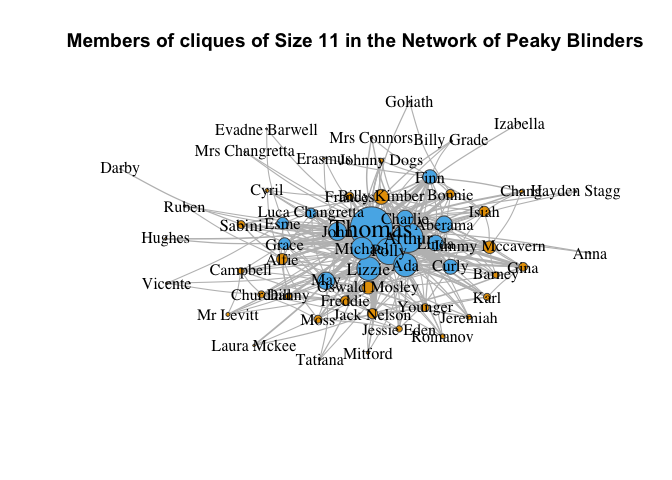
\includegraphics{peakyBlinders_network-part2_files/figure-latex/unnamed-chunk-12-1.pdf}
\#\#\#\# Louvain algorithm

\begin{Shaded}
\begin{Highlighting}[]
\FunctionTok{set.seed}\NormalTok{(}\DecValTok{10}\NormalTok{)}

\NormalTok{communities\_lou }\OtherTok{\textless{}{-}} \FunctionTok{cluster\_louvain}\NormalTok{(peaky\_network)}
\FunctionTok{table}\NormalTok{(}\FunctionTok{membership}\NormalTok{(communities\_lou))}
\end{Highlighting}
\end{Shaded}

\begin{verbatim}
## 
##  1  2  3  4 
## 31 11  9  6
\end{verbatim}

The algorithm found agin four communities, but with different group
sizes. Let's visualise these new groups.

\begin{Shaded}
\begin{Highlighting}[]
\FunctionTok{plot.igraph}\NormalTok{(peaky\_network,}
  \AttributeTok{edge.color =} \StringTok{"gray"}\NormalTok{,}
  \AttributeTok{edge.curved =}\NormalTok{ .}\DecValTok{1}\NormalTok{,}
  \AttributeTok{edge.width =} \DecValTok{1} \SpecialCharTok{+} \FunctionTok{E}\NormalTok{(peaky\_network)}\SpecialCharTok{$}\NormalTok{weight }\SpecialCharTok{/} \DecValTok{15}\NormalTok{,}
  \AttributeTok{vertex.size =} \DecValTok{3} \SpecialCharTok{+} \FunctionTok{degree}\NormalTok{(peaky\_network) }\SpecialCharTok{/} \DecValTok{3}\NormalTok{,}
  \AttributeTok{vertex.frame.color =} \StringTok{"\#555555"}\NormalTok{,}
  \AttributeTok{vertex.label =} \FunctionTok{V}\NormalTok{(peaky\_network)}\SpecialCharTok{$}\NormalTok{name\_edited,}
  \AttributeTok{vertex.color =} \FunctionTok{membership}\NormalTok{(communities\_lou),}
  \AttributeTok{vertex.label.color =} \StringTok{"black"}\NormalTok{,}
  \AttributeTok{vertex.label.cex =} \DecValTok{1} \SpecialCharTok{+} \FunctionTok{betweenness}\NormalTok{(peaky\_network, }\AttributeTok{weights =} \ConstantTok{NA}\NormalTok{) }\SpecialCharTok{/} \DecValTok{1000}\NormalTok{,}
  \AttributeTok{margin =} \FunctionTok{c}\NormalTok{(}\DecValTok{0}\NormalTok{, }\DecValTok{0}\NormalTok{, }\DecValTok{0}\NormalTok{, }\DecValTok{0}\NormalTok{),}
  \AttributeTok{asp =} \DecValTok{0}\NormalTok{,}
  \AttributeTok{layout =}\NormalTok{ layout4,}
\NormalTok{)}
\end{Highlighting}
\end{Shaded}

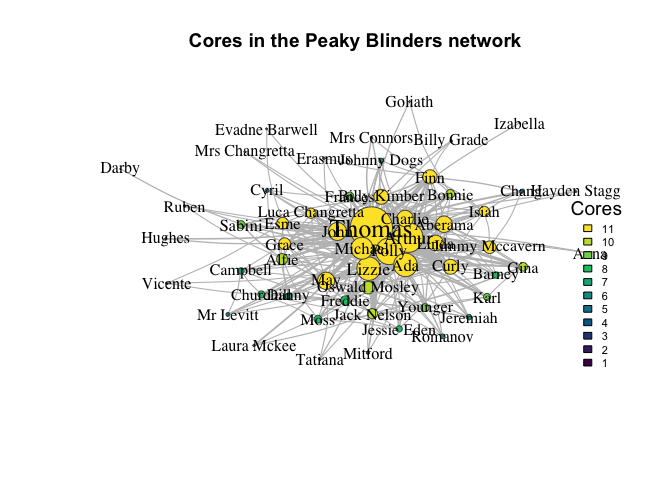
\includegraphics{peakyBlinders_network-part2_files/figure-latex/unnamed-chunk-14-1.pdf}

A confusion matrix can help understand the differences between the two
methods:

\begin{Shaded}
\begin{Highlighting}[]
\FunctionTok{table}\NormalTok{(}\FunctionTok{membership}\NormalTok{(communities\_fg), }\FunctionTok{membership}\NormalTok{(communities\_lou))}
\end{Highlighting}
\end{Shaded}

\begin{verbatim}
##    
##      1  2  3  4
##   1  4  1  4  5
##   2  0 10  0  1
##   3 27  0  1  0
##   4  0  0  4  0
\end{verbatim}

Both node moving algorithms (Fast-Greedy and Louvain) find 4
communities. 27 of the 28 members of Community 3 detected by the Fast
Greedy method are consistently placed in the same community by the
Louvain method, suggesting that these nodes likely form a tightly-knit
or clearly defined cluster within the network, which both algorithms
recognize and consistently categorize. Similarly, 10 nodes out of eleven
from Fast Greedy's Community 2 were placed together by the Louvain
algorithm.

Nevertheless, the confusion matrix shows some differences between the
two algorithms' assignments. For instance, for Community 1 of Fast
Greedy, the nodes are spread across four different communities in the
Louvain method. This indicates that the cohesion within this group as
perceived by the Fast Greedy method is not as strong under the criteria
used by the Louvain algorithm.

\hypertarget{infomap-community-detection-algorithm}{%
\paragraph{InfoMAP community detection
algorithm}\label{infomap-community-detection-algorithm}}

Rather than optimising modularity, InfoMAP minimises the expected
description length of a random walker trajectory. In other words, the
partition into communities is done so that walks should spend longer
time within communities than between.

\begin{Shaded}
\begin{Highlighting}[]
\NormalTok{communities\_infomap\_unweighted }\OtherTok{\textless{}{-}} \FunctionTok{cluster\_infomap}\NormalTok{(peaky\_network, }\AttributeTok{e.weights =} \ConstantTok{NULL}\NormalTok{)}
\NormalTok{communities\_infomap }\OtherTok{\textless{}{-}} \FunctionTok{cluster\_infomap}\NormalTok{(peaky\_network)}
\FunctionTok{table}\NormalTok{(}\FunctionTok{membership}\NormalTok{(communities\_infomap\_unweighted))}
\end{Highlighting}
\end{Shaded}

\begin{verbatim}
## 
##  1 
## 57
\end{verbatim}

\begin{Shaded}
\begin{Highlighting}[]
\FunctionTok{table}\NormalTok{(}\FunctionTok{membership}\NormalTok{(communities\_infomap))}
\end{Highlighting}
\end{Shaded}

\begin{verbatim}
## 
##  1 
## 57
\end{verbatim}

Interestingly, community detection with InfoMAP (weighted and
unweighted) results in a single community. This is an indication that
the flow of interactions between characters does not significantly
bottleneck at any point that would otherwise suggest the presence of
distinct groups.

When contrasted with the outputs from the previous algorithms, which
identified multiple communities, the result from InfoMAP might indicate
that the network is overall tightly-knit but contains subtler structures
that are more sensitive to the parameters and methods of node-moving
algorithms.

\hypertarget{compare-louvain-algorithm-and-grouping-by-origin}{%
\paragraph{Compare Louvain algorithm and grouping by
origin}\label{compare-louvain-algorithm-and-grouping-by-origin}}

\begin{Shaded}
\begin{Highlighting}[]
\FunctionTok{sort}\NormalTok{(}\FunctionTok{membership}\NormalTok{(communities\_lou))}
\end{Highlighting}
\end{Shaded}

\begin{verbatim}
##            finn          arthur          thomas           danny         charlie 
##               1               1               1               1               1 
##           grace            john           curly          lizzie         erasmus 
##               1               1               1               1               1 
##            esme            anna           linda         vicente         romanov 
##               1               1               1               1               1 
##          hughes        izabella         frances          bonnie           isiah 
##               1               1               1               1               1 
##         goliath           chang          barney         mitford    billy_kimber 
##               1               1               1               1               1 
##     johnny_dogs     mrs_connors  evadne_barwell     billy_grade  mrs_changretta 
##               1               1               1               1               1 
##    hayden_stagg       churchill         freddie           polly             ada 
##               1               2               2               2               2 
##        campbell         younger        jeremiah            moss            karl 
##               2               2               2               2               2 
##         aberama     jessie_eden             may         michael         tatiana 
##               2               2               3               3               3 
##            gina  jimmy_mccavern   oswald_mosley     jack_nelson     laura_mckee 
##               3               3               3               3               3 
##       mr_levitt           alfie          sabini           ruben           darby 
##               3               4               4               4               4 
##           cyril luca_changretta 
##               4               4
\end{verbatim}

\begin{Shaded}
\begin{Highlighting}[]
\FunctionTok{table}\NormalTok{(}\FunctionTok{V}\NormalTok{(peaky\_network)}\SpecialCharTok{$}\NormalTok{origin, }\FunctionTok{membership}\NormalTok{(communities\_lou))}
\end{Highlighting}
\end{Shaded}

\begin{verbatim}
##             
##               1  2  3  4
##   Birmingham 19  9  1  1
##   Ireland     4  1  1  0
##   London      2  1  3  3
##   New York    2  0  2  1
##   Other       2  0  1  1
##   Russia      2  0  1  0
\end{verbatim}

Cross-tabulating the communities detected by the algorithm and character
groupings by their city or country of origin yields interesting results.
Although modularity alone had hinted that origin might not be a decisive
factor for tie formation, there are some overlaps with the community
attribution made by the Louvain algorithm.

\begin{itemize}
\item
  Community 1 predominantly consists of characters from Birmingham (19
  out of 31), suggesting that this community could represent the central
  group of characters based in Birmingham, likely reflecting the primary
  setting and central figures Peaky Blinders. Unsurprinsingly, all men
  of the Shelby family are in this community (Thomas, Arthur, Finn,
  John), as well as their trusted officers (Danny, Curly, Johnny Dogs)
\item
  The other community mostly constituted of characters originating from
  Birmingham is Community 2 (9 out of 11). Interestingly, this second
  Birmingham-related community includes the most influential women in
  the Shelby family, such as Polly, the matriarch (along with her lover
  Aberama). In fact, from the Shelby siblings, all men are in Community
  1, and the only woman, Ada, is isolated in Community 2 (along with her
  husband, Freddie, and son, Karl). These findings suggests that gender
  may indeed have a role in the creation of ties, along with family
  ties.
\item
  93\% of the characters from Birmingham are in either Community 1 or 2.
  Community 3 and Community 4 appear to be smaller and more diverse in
  terms of character origin. Community 4 has a slight concentration of
  characters from London (3 out of 6). However, this community seems to
  be constituted along narrative lines. Indeed, five of its members
  (Alfie and his dog Cyril, Sabini, Darby and Luca Changretta) are major
  antagonists of Peaky Blinders.
\item
  Finally, Community 3 is the most diverse, including characters from
  all origins, and possibly hinting at more internationally connected
  narratives or character interactions. For example, although Michael
  originates from Birmingham, he marries Gina and moves to New York,
  where she is from, to conducts business with her uncle Jack Nelson,
  therefore connecting two continents through his interactions.
\end{itemize}

Overall, the Louvain community detection algorithm has uncovered
communities in the narrative of Peaky Blinders, hidden when only
considering single attributes at a time, but seemingly driven by
interactions based on a set of factors including place of origin,
gender, family or business.

\hypertarget{small-world-and-scale-free-networks}{%
\subsection{Small-world and scale-free
networks}\label{small-world-and-scale-free-networks}}

\begin{itemize}
\tightlist
\item
  \textbf{Scale-free network}: In a scale-free network, most nodes have
  only a few connections, while a small number of nodes - often referred
  to as ``hubs'' - have a much large number of connections. A scale-free
  network is characterised by its highly uneven distribution of
  connections among the nodes. Specifically, this distribution follows a
  follows a power law, meaning that the probability of observing an node
  with `x' connections decays as x increases: typically in the form P(x)
  = Cx\^{}-α, with normalisation constant C and power law exponent α.
\end{itemize}

The power law is ubiquitous in nature and society, let's observe whether
it characterises the interactions of Peaky Blinders characters.

First, degree distribution

\begin{Shaded}
\begin{Highlighting}[]
\NormalTok{degree\_data }\OtherTok{\textless{}{-}} \FunctionTok{degree\_distribution}\NormalTok{(peaky\_network, }\AttributeTok{cumulative =} \ConstantTok{FALSE}\NormalTok{)}
\NormalTok{cumulative\_degree\_data }\OtherTok{\textless{}{-}} \FunctionTok{degree\_distribution}\NormalTok{(peaky\_network, }\AttributeTok{cumulative =} \ConstantTok{TRUE}\NormalTok{)}

\NormalTok{degree\_df }\OtherTok{\textless{}{-}} \FunctionTok{data.frame}\NormalTok{(}
  \AttributeTok{degree =} \FunctionTok{seq\_along}\NormalTok{(degree\_data) }\SpecialCharTok{{-}} \DecValTok{1}\NormalTok{, }
  \AttributeTok{probability =}\NormalTok{ degree\_data)}

\NormalTok{cumulative\_degree\_df }\OtherTok{\textless{}{-}} \FunctionTok{data.frame}\NormalTok{(}
  \AttributeTok{degree =} \FunctionTok{seq\_along}\NormalTok{(cumulative\_degree\_data) }\SpecialCharTok{{-}} \DecValTok{1}\NormalTok{, }
  \AttributeTok{probability =}\NormalTok{ cumulative\_degree\_data)}

\NormalTok{p1 }\OtherTok{\textless{}{-}} \FunctionTok{ggplot}\NormalTok{(degree\_df, }\FunctionTok{aes}\NormalTok{(}\AttributeTok{x =}\NormalTok{ degree, }\AttributeTok{y =}\NormalTok{ probability)) }\SpecialCharTok{+}
  \FunctionTok{geom\_line}\NormalTok{() }\SpecialCharTok{+}
  \FunctionTok{geom\_point}\NormalTok{() }\SpecialCharTok{+}
  \FunctionTok{labs}\NormalTok{(}\AttributeTok{title =} \StringTok{"Degree Distribution"}\NormalTok{, }\AttributeTok{x =} \StringTok{"Degree"}\NormalTok{, }\AttributeTok{y =} \StringTok{"p(degree)"}\NormalTok{) }\SpecialCharTok{+}
  \FunctionTok{theme\_minimal}\NormalTok{()}

\NormalTok{p2 }\OtherTok{\textless{}{-}} \FunctionTok{ggplot}\NormalTok{(cumulative\_degree\_df, }\FunctionTok{aes}\NormalTok{(}\AttributeTok{x =}\NormalTok{ degree, }\AttributeTok{y =}\NormalTok{ probability)) }\SpecialCharTok{+}
  \FunctionTok{geom\_line}\NormalTok{() }\SpecialCharTok{+}
  \FunctionTok{geom\_point}\NormalTok{() }\SpecialCharTok{+}
  \FunctionTok{labs}\NormalTok{(}\AttributeTok{title =} \StringTok{"Cumulative Degree Distribution"}\NormalTok{, }\AttributeTok{x =} \StringTok{"Degree"}\NormalTok{, }\AttributeTok{y =} \StringTok{"p(degree)\textgreater{}x"}\NormalTok{) }\SpecialCharTok{+}
  \FunctionTok{theme\_minimal}\NormalTok{()}

\CommentTok{\# Combining the plots side by side}
\FunctionTok{grid.arrange}\NormalTok{(p1, p2, }\AttributeTok{ncol =} \DecValTok{2}\NormalTok{)}
\end{Highlighting}
\end{Shaded}

\includegraphics{peakyBlinders_network-part2_files/figure-latex/unnamed-chunk-18-1.pdf}

These plots hint at a potential power law distribution of degree. When
picking a random node in the network, it has the highest probability of
having a degree between 0 and 10, with a maximum at 3. Conversely, only
a few nodes have especially high degrees (one at 54, and four others at
30 or above).

\begin{Shaded}
\begin{Highlighting}[]
\CommentTok{\# Remove zero probability \& degree for log scale}
\NormalTok{degree\_log\_df }\OtherTok{\textless{}{-}}\NormalTok{ degree\_df[degree\_df}\SpecialCharTok{$}\NormalTok{probability }\SpecialCharTok{\textgreater{}} \DecValTok{0} \SpecialCharTok{\&}\NormalTok{ degree\_df}\SpecialCharTok{$}\NormalTok{degree }\SpecialCharTok{\textgreater{}} \DecValTok{0}\NormalTok{, ]}

\NormalTok{cumulative\_degree\_log\_df }\OtherTok{\textless{}{-}}\NormalTok{ cumulative\_degree\_df[cumulative\_degree\_df}\SpecialCharTok{$}\NormalTok{probability }\SpecialCharTok{\textgreater{}} \DecValTok{0} \SpecialCharTok{\&}\NormalTok{ cumulative\_degree\_df}\SpecialCharTok{$}\NormalTok{degree }\SpecialCharTok{\textgreater{}} \DecValTok{0}\NormalTok{, ]}

\NormalTok{log\_log\_degree\_plot }\OtherTok{\textless{}{-}} \FunctionTok{ggplot}\NormalTok{(degree\_log\_df, }\FunctionTok{aes}\NormalTok{(}\AttributeTok{x =}\NormalTok{ degree, }\AttributeTok{y =}\NormalTok{ probability)) }\SpecialCharTok{+}
  \FunctionTok{geom\_point}\NormalTok{() }\SpecialCharTok{+}
  \FunctionTok{geom\_line}\NormalTok{() }\SpecialCharTok{+}
  \FunctionTok{scale\_x\_log10}\NormalTok{() }\SpecialCharTok{+}
  \FunctionTok{scale\_y\_log10}\NormalTok{() }\SpecialCharTok{+}
  \FunctionTok{labs}\NormalTok{(}\AttributeTok{title =} \StringTok{"Degree Distribution (Log{-}Log)"}\NormalTok{, }\AttributeTok{x =} \StringTok{"Degree (log scale)"}\NormalTok{, }\AttributeTok{y =} \StringTok{"p(degree) (log scale)"}\NormalTok{) }\SpecialCharTok{+}
  \FunctionTok{theme\_minimal}\NormalTok{()}

\NormalTok{log\_log\_cumulative\_plot }\OtherTok{\textless{}{-}} \FunctionTok{ggplot}\NormalTok{(cumulative\_degree\_log\_df, }\FunctionTok{aes}\NormalTok{(}\AttributeTok{x =}\NormalTok{ degree, }\AttributeTok{y =}\NormalTok{ probability)) }\SpecialCharTok{+}
  \FunctionTok{geom\_point}\NormalTok{() }\SpecialCharTok{+}
  \FunctionTok{geom\_line}\NormalTok{() }\SpecialCharTok{+}
  \FunctionTok{scale\_x\_log10}\NormalTok{() }\SpecialCharTok{+}
  \FunctionTok{scale\_y\_log10}\NormalTok{() }\SpecialCharTok{+}
  \FunctionTok{labs}\NormalTok{(}\AttributeTok{title =} \StringTok{"Cumulative Degree Distribution }\SpecialCharTok{\textbackslash{}n}\StringTok{(Log{-}Log)"}\NormalTok{, }\AttributeTok{x =} \StringTok{"Degree (log scale)"}\NormalTok{, }\AttributeTok{y =} \StringTok{"p(degree)\textgreater{}x (log scale)"}\NormalTok{) }\SpecialCharTok{+}
  \FunctionTok{theme\_minimal}\NormalTok{()}

\NormalTok{log\_log\_cumulative\_plot}
\end{Highlighting}
\end{Shaded}

\includegraphics{peakyBlinders_network-part2_files/figure-latex/unnamed-chunk-19-1.pdf}
The log-log plot of the cumulative degree distribution is a key
visualization for analyzing the scale-free characteristics of a network.
The beginning part of the cumulative degree distribution curve seems to
follow a rough linear pattern in the log-log scale, suggesting a
power-law regime typical for scale-free networks. Although towards the
higher degrees, there appears to be more variation and a potential
drop-off. This could indicate that while the network does exhibit
scale-free characteristics for a range of degrees, it does not strictly
follow a power-law distribution across all degrees, which could be due
to the relatively small size of the network.

Several mechanisms can lead to the formation of scale-free networks,
most of them are usually driven by some form of feedback loop. For
example, preferential attachment - when new nodes prefer to attach to
nodes that are already well-connected - and duplication are two of such
mechanisms. A network of TV series character interactions is a special
case because its interactions are solely driven by choices of the
screenwriter to advance the plot, not by decisions made by the nodes
themselves.

The apparent scale-free characteristics observed in this network are
therefore the manifestation of the structure of the series, centered
around a few characters. The development of the power law distribution
is caused by the need to advance the plot around the Shelby family, and
side characters do not need to interact amongst each other. As the story
advances and the network grows further, it could be expected that its
scale-free proporty would be enhanced, as side or deceased characters,
and antagonists from previous seasons stop appearing in the show and
therefore cannot interact at all with new characters.

\begin{itemize}
\tightlist
\item
  \textbf{Small-world phenomenon}: The small-world phenomenon refers to
  the property of a network wherein most nodes can be reached from every
  other node by a small number of steps, despite the network being very
  large. It is often quantified with a low average shortest path length,
  and is most likely to be exhibited by networks whose edges are mostly
  formed at random.
\end{itemize}

Report the degree distribution in your network and some measures of
distance between the nodes in your network. Discuss if your network
looks like a scale-free network and exhibits small-world characteristics
(Your network will likely be rather small to discuss these properties
which apply to very large networks. But imagine you expand your network
by adding many more nodes or by collecting additional data from many
other similar networks. Would you expect to see scale- free or
small-world network characteristics?). Briefly discuss the mechanism
that may or may not result in a scale-free and a small-world network in
your case.

\hypertarget{exponential-random-graph-modelling-ergm}{%
\subsection{Exponential random graph modelling
(ERGM)}\label{exponential-random-graph-modelling-ergm}}

\end{document}
